% This is samplepaper.tex, a sample chapter demonstrating the
% LLNCS macro package for Springer Computer Science proceedings;
% Version 2.20 of 2017/10/04
%
\documentclass[runningheads]{llncs}
%
\usepackage{graphicx}

\usepackage{amsmath}
\usepackage{amssymb}
\usepackage{hyperref} 
\usepackage{soul}  
\usepackage{color}
\usepackage{xcolor}
\usepackage{graphicx}
\usepackage{inputenc} 
\usepackage{comment}
%\usepackage{wrapfig} 
\usepackage{ae}  
\usepackage{sidecap}
\usepackage{url}
\usepackage[T1]{fontenc} 
\usepackage{verbatim}
\usepackage{listings} 
\usepackage{tikz}
\usepackage{etoolbox}
\usepackage{mdframed}
\usepackage{tabularx}
\usepackage{multirow}
\usepackage{setspace}

\newenvironment{code}
    {\noindent
     \rule{\columnwidth}{0.6pt}
     \vspace{-4mm}
     \scriptsize \verbatim}
    {\endverbatim \normalsize
     \vspace{-4mm} 
    \rule{\columnwidth}{0.6pt} 
 	}
\usepackage{wrapfig}
\usepackage{relsize}
\usepackage{microtype}
\usepackage{multirow}
\usepackage{semantic}

\usepackage{booktabs}
\usepackage{paralist}
% important for nicer code font
\usepackage[scaled]{beramono}

\definecolor{lightlightgray}{gray}{0.9}
\definecolor{codecolor}{gray}{0.15} 
\definecolor{javadocblue}{rgb}{0,0,0.8} % javadoc
\definecolor{blackblack}{rgb}{0,0,0}
  
\definecolor{myGray1}{rgb}{0.85,0.85,.85}

\lstset{
basicstyle=\ttfamily\scriptsize\color{codecolor}, 
keywordstyle=\color{blackblack}\bfseries,       
% keywordstyle=\color{javadocblue},     
commentstyle=\color{gray},              
numbers=none,                           
numberstyle=\tiny,                      % Line-numbers fonts
stepnumber=1,                           % Step between two line-numbers
numbersep=5pt,                          % How far are line-numbers from code
%backgroundcolor=\color{lightlightgray}, % Choose background color
tabsize=2,     
frame=single,
%xleftmargin=1.5mm,
%xrightmargin=1.5mm,
captionpos=b,   
keepspaces=true,
xleftmargin=1.5mm,
xrightmargin=1.5mm,                        % Caption-position = bottom
breaklines=true,    
escapeinside={@}{@},
                    % Automatic line breaking?
breakatwhitespace=false,                % Automatic breaks only at whitespace?
showspaces=false,                       % Dont make spaces visible
showtabs=false,                         % Dont make tabls visible
columns=flexible,                       % Column format
morekeywords={}
mathescape=false
} 


% Used for displaying a sample figure. If possible, figure files should
% be included in EPS format.
%
% If you use the hyperref package, please uncomment the following line
% to display URLs in blue roman font according to Springer's eBook style:
% \renewcommand\UrlFont{\color{blue}\rmfamily}

\newcommand\parhead[1]{\vspace{1mm}\noindent\textbf{{#1}}\ \ }  
\newcommand\parheadX[1]{\vspace{-1.0mm}\noindent\textbf{{#1}}\ \ }  

\newcommand{\toolurl}[1]{\footnote{\smaller\url{{#1}}\normalsize}}
\newcommand{\ic}[1]{\changefont{cmtt}{m}{n}{#1}\normalfont}  % inline code
\newcommand{\changefont}[3]{\fontfamily{#1}\fontseries{#2}\fontshape{#3}\selectfont}
\newcommand{\fig}[1]{Fig. \ref{#1}}  % inline code
\newcommand{\sect}[1]{Sec. \ref{#1}}  % inline code


\newcommand\todo[1]{\vspace{1mm}\noindent\textbf{\color{red} {{TODO: {#1}} }}}  


\newmdenv[innerlinewidth=1pt, linecolor=black, innerleftmargin=3pt,
innerrightmargin=3pt,innertopmargin=3pt,innerbottommargin=3pt,backgroundcolor=lightlightgray]{mybox}

\newif\ifFullVersion
\FullVersionfalse

\begin{document}
%
\title{Programming \\ vs. \\ That Thing Subject Matter Experts Do}

\titlerunning{Programming vs. SME'ing}

%  \titlerunning{Abbreviated paper title} If the paper title is too long for the
% running head, you can set an abbreviated paper title here
\author{Markus Voelter}
\authorrunning{M. Voelter}
% First names are abbreviated in the running head.
% If there are more than two authors, 'et al.' is used.
\institute{independent/itemis, Oetztaler Strasse 38, 70327 Stuttgart, Germany\\
\email{voelter@acm.org}}
\maketitle              % typeset the header of the contribution
\begin{abstract}
\keywords{Domain Specific Language  \and End-user Programming \and Language Engineering.}
\end{abstract}
%
%
%

% \begin{mdframed}
% \textbf{A note for the ISOLA reviewers.} In my experience, one of the biggest challenges
% of the DSL community is that we have a very hard time convincing people who
% might benefit from using DSLs to actually use one.
% We have all written lots of scientific papers and case studies that demonstrate
% clearly that DSLs are useful, but still we have a hard time breaking through. With
% this paper I'm trying a different approach. It is based on anecdotes, it is hopefully
% easy to read, and it doesn't contain any technical details or data.
% I know that this is not a very
% scientific approach. But I would ask you to read the paper and provide feedback
% relative to the goal: to try and convince programmers to give DSLs a try.
% Because---again---I think this is really what our community needs to move forward.
% \end{mdframed}

\newcommand{\datev}{DATEV}
\newcommand{\voluntis}{Voluntis}
\newcommand{\ohb}{OHB}

\newcommand{\caseend}{$\blacksquare$}

 


\section{The role of subject matter experts}

Subject matter experts, or SMEs, own the knowledge and expertise that is the
backbone of software and the foundation of digitalization. But too often this
rich expertise is not captured in a structured way and gets lost when
translating it for software developers for implementation. With the rate of
change increasing, time-to-market shortening and product variability blooming,
this indirect approach of putting knowledge into software is increasingly
untenable. It causes delays, quality problems and frustration for everybody
involved. A better approach is to empower \emph{subject matter experts} to
capture, understand, reason about data, structures, rules, behaviors and other
forms of knowledge and expertise in a precise and unambiguous form by providing
them with tailored software languages and tools that allow them to directly
edit, validate, simulate and test that knowledge. The models created this way
are then automatically transformed into program code. The \emph{software
engineers} focus their activities on building these languages, tools and
transformations, plus robust execution platforms for the generated code.

\todo{Refer to Manifesto when it is done}

\section{(Where) Does this work?}

Building the necessary tooling and automation requires investment, and this
investment must pay off for it to make economical sense. This is why the
approach only works in domains that have the following characteristics. First,
the subject matter that goes into the software has to have a minimum
\textbf{size} and degree of \textbf{complicatedness}. Often this means that
there are people in the company who consider themselves the \textbf{experts} in
that subject matter. It's they who everybody asks about specifics in the domain.
The second criterion is that this subject matter itself will remain
\textbf{relevant over time} and that the business intends to stay in that domain
for a reasonably long time. Finally, even though the subject matter as a whole
is relevant for a long time, a degree of \textbf{evolution} or \textbf{variety}
is usually needed. We have seen this approach used in the following domains, among others:

\parhead{In insurances,} DSLs are used by insurance product definition~\cite{zurich} staff to develop a
variety of ever evolving insurance products. With increased differentiation
between products, these become more and more complicated while at the same time
increasing in variety. The company itself is in the insurance business for the
long run. [Reference to detailed case study coming once MPS book is published\todo{}]

\parhead{In healthcare,} DSLs are used by doctors and other healthcare
professionals to develop digital therapeutics algorithms. The company wants to
grow over a decade and develop many of these algorithms. The subject matter is
large and complicated because it captures medical expertise. Details about
the French-American company Voluntis see \cite{voelter2019vol}.

\parhead{In public adminstration,} as government agencies, they are certainly in
it for the long run, while legislation for public benfits and tax calculation
changes and evolves regularly. The agencies are full of experts who interpret
and understand the law. On the other side, the service providers who develop
software for tax advisors has the same challenges and uses DSLs as well.
[Reference to detailed case study coming once MPS book is published\todo{}]

\parhead{In payroll,} the applicable regulations that govern the  
deducations from an employee's gross salary and the additional taxes and fees
they have to pay are just as complicated, long-lasting and ever changing as tax
law. Service provides who develop payroll software therefore also whole 
departments full of experts and benefit from DSLs. 
[Reference to detailed case study coming once MPS book is published\todo{}]

\vspace{3mm}

\noindent For an overview over this idea and a couple of easily readable 
case studies, see my InfoQ article~\cite{infoq}.

\section{Can SMEs do that?}

In my experience, based on the experiences mentioned above, plus a few more, the
answer to the question in the title of this section, \emph{can they do that}, is
a clear yes. At least this is true for the majority of subject matter experts I
have worked with. But a key question is: to what extent do the subject matter
experts who use our DSLs and tools have to become programmers? Do they have the
\emph{skills} to be programmers (hint: most don't). Do they \emph{want} to
become programmers (hint: most don't). But we still expect them to use
``languages'' and IDE-like tools. So:

\vspace{2mm}
\noindent \textbf{Which parts of what we call programming do they have to learn?
How is SME'ing different from programming, and where does it overlap?}
\vspace{2mm}

\noindent In the next section, the main part of this paper, I will try to provide some
insight.

\section{Difference between programming and SME'ing}



\subsection{Skills and Responsibilities}

\begin{figure}
\begin{center}
    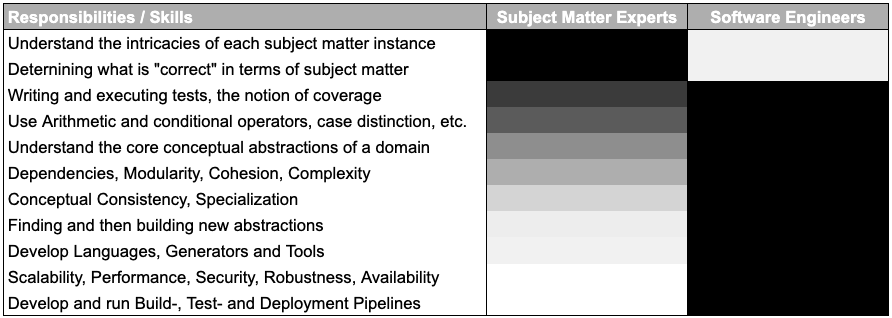
\includegraphics[width=1\columnwidth]{figures/table-respo.png}
    \caption{Comparing programming (what software engineers do) from
    whatever not-yet-named activity subject matter experts should do to 
    directly contribute to software. Darker shade means ``is more relevant''.}
    \label{table-respo}
\end{center} 
\end{figure} 

\fig{table-respo} shows the differences in responsibilities of software
develoeprs and SMEs. The darker the shade, the more responsibility the
respective community has for that concern. Let's start our discussion
with the two black and white cases, those where there is no overlap.
There's probably no disagreement about these.

\parhead{Region 1, SME only} Let's start with region 1, which is completely the
responsibility of SMEs. They have to understand every particular example, case,
situation, exception of the subject matter they are describing with the DSL.
This is their natural responsibility, this is why they exist. SEs on the other
side should not have to care at all. Again, this separation is the reason for
using DSLs and tools in the first place. Related to this, the SMEs are also in
charge of determining what consistutes correct behavior in the subject matter.
They take responsibility for what should go into test cases.

\parhead{Region 2, SE only} Let's move on to region 2, which is completely the
responsibility of SEs.
Building and operating automated CI pipelines that include building, packaging
and running tests is nothing the SME should be concerned with, except maybe
getting emails if tests fail (after they have run correctly in their local
environment, otherwise they should never reach the CI server).
 
The same is true for taking care of performance, scalability, 
safety, security, robustness and availability, all the operational
(aka non-functional) concerns of the final software system. Keeping the
subject matter segregated from these technical aspects of software is
a key benefit of the approach, and it is clear that this should be 
handled in platforms, frameworks and code generators -- all clearly
the domain of SEs.

Finally, the development of the DSLs and tools that will then be used
by the SMEs for capturing, analysing and experimenting with subject matter
is the responsibility of software people. It might not be the domain of
all of the software engineers, but maybe that of a certain specialization
called language engineer. Also, a very few of the subject matter experts,
we sometimes refer to them as gurus, of course have to help survey,
understand, analyse and abstract the domain so that the language engineers
can build the languages. But the regular SME, the dozens or hundreds
that many of our customers employ, are not involved with this task.

\parhead{Region 3, Testing} Let's now look at region 3, one that apparently has
shared complete responsibility. It's a bit misleading. Indeed, both communities
have to understand the purpose of testing, what a test case is, and appreciate
the notion of coverage, i.e., understanding when they have enough tests to be
(reasonably) sure that there are no more (reasonably few) bugs in the logic. But
of course the SMEs care about this \emph{only} for subject matter (on DSL/model
level) whereas the SEs care about it only in the platform, frameworks and
generators. So they both have to understand the concept of testing, but there
are no artifacts for which they have shared responsibility.

\parhead{Region 4, shared skills} We are now ready to look at the interesting
part, region 4. All of the things in this region are things that are completely
at home in programming and software engineering. So SEs care. But they are also
relevant, to different degrees, to SMES. Let's explore them in detail.

Of course the SMEs have to understand the conceptual abstractions of the domain.
Otherwise they cannot use the language.
Understanding abstractions is not easy in general, but because in a DSL these
abstractions are closely aligned with the subject matter, the subject matter
experts -- in my experience -- are able to understand it. Maybe not every little
detail (which is why the box is dark grey and not black) but sufficiently. The
SEs have to understand these abstractions as well, especially the language
engieneers. 

A note: the fact that there is shared understanding about the core abstractions
of the subject matter in which the SMEs and the SEs co-create software is a major
reason why DSLs are so useful here. The language definition, and its conceptual
cousins, the core abstractions, are a great unambiguous and clearly-scoped
foundation for productive collaboration.

No real-world subject-matter focused DSL I have every seen can be used or
understood without understanding the notion of values, and some notion of
functions. It doesn't matther whether we're talking specifically about (textual)
functions, (Excel-style) decision tables or (graphical) dataflow diagrams. The
good thing is that essentially everybody has come across these at school or
at university, so this is usually not a huge challenge. Another very fundamental
concept that everybody should understand is the notion of mutable state
as expressed by state transition systems (aka state charts or state machines).

Similarly, the understanding of dot expression to mean ``the member X of entity
Y'' or ``do Z with entity Y'' is very hard to avoid, because working with parts
of things or performing activities on things is almost unavoidable. For many
SMEs, this is harder to get used to. We've experimented with literally writing
\ic{member of object} instead of \ic{object.member} but this is hard to do 
because of scoping. In the latter, you can easily scope the code completion
menus to members of \ic{object} because you write the object first, whereas
in the former case the code completion for the member has to show all members
of all objects.

Another set of constructs that is hard to do without is arithmetic, logcial
and and comparison operators (together with types like number or Boolean), 
again independent of their concrete syntax (text, symbol or graphical). Again,
luckily, most SMEs remember those from school or university. So this is also
not a big challenge. The same is true for the notion of a conditional, such
as \ic{if \ldots then} or \ic{switch\{case, case, case\}}. 

The reason why these two lines are grey for SMEs and not totally black is
because the complexity in the expressions built with these language concepts
should (and usually can) be kept lower for SMEs. For example, for complicated
decisions, we can support graphical decision tables of various forms which are
much easier to grasp then nested \ic{if} statements and the like. 

Several of the DSLs I have built require an understanding of the notion of
parametrization. For example, in a function-like thing, the values passed into
the call are mapped (by position or by name) to formal arguments that are then
processed in the body of the function. Most SMEs have no problems with this
-- again, school experience -- but some do. In my experience this is the 
threshold where the need for education and training starts (beyond building
the shared understanding about the core concepts of a domain). A related
concept is the notion of instantiation, where, usually, the instance has
independent values for its state and its evolution. This is not taught in
school, and it's not taught outside of computer science at university, so
training is needed. On the other hand, many DSLs don't need this, which is
why this box is a lighter shade of gray.

We're getting to more advanced concepts that are harder to grasp for many SMEs,
but they are also not necessary in all DSLs (though unavoidable in some
domains). The notion of specialization or subtyping is key here. While everybody
understand subtyping intuitively (``an eagle \emph{isa} bird \emph{isa} animal
\emph{isa} living thing \emph{isa} object''), many SMEs struggle with the
consequences. Especially the mental assembly of everything that's in a subtype
by (mentally) going through all its supertypes is hard: ``we're not seeing
the big picture'' is what I often hear. Practice helps, but so can tools that
optionally show all the inherited stuff inline in the subtype's definition.

For complex subject matter -- the tax stuff comes to mind -- the models created
with the DSLs become larger, and complexity often rises along with the size.
Notions like reduction of unnecessary dependencies, module boundaries,
interfaces, and more generally, cohesion and coupling become an issue. Most SMEs
struggle here. But on the other hand, 95\% of the work of an SME can proceed
without caring about these things, except during initial design or downstream
review phases, where SE or guru involvement is often needed so sort things out.

The final ingredient in region 4 is discovering and then defining new
abstractions. Usually not the strong suit of SMEs. Those that are able to
do this are usually the gurus we talked about before, or they have been
assimilated wholly but the software development team. But luckily it is
quite rare that SMEs are required to define new abstractions, because those
that are relevant should be available first-class in the DSL -- or retrofitted
for the next version once the need becomes obvious. Many of our DSLs are
funclarative~\cite{voelter2018fusing} where small, simple calculations are done with a functional
language (so users don't have to care about effects at this level) and 
when things get more complicated, we add declarative first-class concepts
to the language.
 
\begin{figure}
\begin{center}
    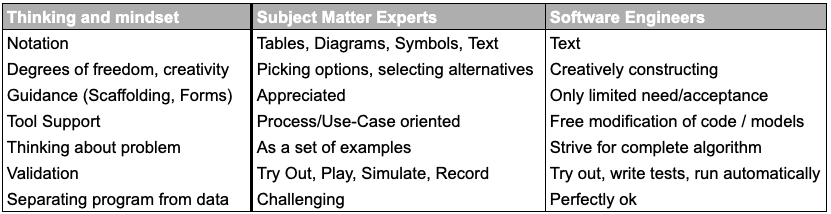
\includegraphics[width=1\columnwidth]{figures/table-prefs.png}
    \caption{SMEs make different trade-offs than software engineers 
    regarding the languages and tools they want to work with.}
    \label{table-prefs}
\end{center} 
\end{figure} 

\subsection{Different Emphasis}

In my experience, (most) SMEs prioritize the features of languages and IDEs differently
from (most) developers. In this section we'll look at some of the more prominenet differences.
\fig{table-prefs} summarizes the differences.

\parhead{Notation} Developers prefer textual notations, both for its
conciseness, but also for its homogeneity with regards to storing, editing,
diffing and merging programs. SMEs tend to emphasize readability and fit of
the notation with establised representations in the domain (e.g., tables in
the tax law documents) over these efficiency concerns. Therefore, if you can
build DSLs that are more diverse in notation -- and not just colored text with
curly braces and nesting -- SME buy-in is usually easier to get.

\parhead{Selecting vs. Creating} Developers love the creative freedom of coming
up with an algorithm, crafting their own suitable abstractions from small,
flexible building blocks. SMEs -- including because of their often limited
abstraction skills -- prefer picking from options, selecting alternatives.
In my experience it is ok for them if they have to read a bit more documentation
that (hopefully!) explains what the different options or alternatives mean.
So DSLs often rely on first-class concepts for the various needs of the domain,
even if this requires the users to first understand what these mean
specifically. The approach is usually also benefitial for domain-related
semantic analysis (more first class content makes it easier to analyze) and it's
easier to have a good notation (because you can associate specific notations
with these first-class concepts). In contrast, programming languages emphasize
orthogonality and flexibility of their first-class concepts.

\parhead{Guidance} A related topic is guidance. Developers are happy with
opening an empty editor and starting to write code. Code completion guides
them a little bit. SMEs prefer more guidance, almost to the point where 
template-models are pre-created after selection from a menu. DSLs that feel
like a mix between a form-based application and program code seem to be 
particularly appreciated in many contexts.

\parhead{Tool Support} Thinking this further, SEs prefer a toolbox approach
to tooling: the tool gives you 5 million different tools to do things. It's
the developer's job to use the tool at the right time, in the right way.
SMEs are more use-case oriented. They want tool support for their typical
process steps, and specific tool support for them. We have built DSLs that
included wizard-like functionality in the IDE where using the wizard required
more input gestures than just code-completion supported typing. Still the
wizard was preferred by the SMEs.
 
\parhead{Thinking about problems} It's almost a defining feature of programmers
that they think about a problem (and its solution) as a complete algorithm
that can cover all possible execution paths. Sure, tests then validate 
specific scenarios, but developers \emph{think} in algorithms. SMEs often
think in terms of examples first, and sometimes only. For example, it is easier
for them to deal with a (hopefully complete) set of sequence diagrams rather
than with a state machine. In terms of DSL design this means that more
emphasis on case distinction where the various scenarios can be specified
separately (even if this incurs a degree of code duplication) is often 
a good idea.

\parhead{Validation} Most developers are good at writing tests, writing
them against APIs on a relatively small unit size, and then running these
tests automatically all the time. SMEs often think of validation more in
terms of ``playing with the system''. They prefer ``simulation GUIs'' over
writing repeatable tests as (a different kind of) program. So build those
simulators first, and then allow the simulator to record ``play sessions''
and persist them as generated test cases for downstream reexecution.

\parhead{Recipe vs. Execution} A program is a recipe which, when combined
with input data, behaves in a particular way. That behavior depends on the
input data. So whenever SEs write code, they continuously imagine (and sometimes
try our or trace with the debugger) how the program behaves for (all possible
combinations of) input data. Many SMEs are not very good (practiced) at doing
this. One reason why Excel is so popular is because it does not make this
distinction between program and data: the program always runs (or, alternatively,
a spreadsheet never runs, it just ``is''). So anything from the universe of
live programming is helpful.

\vspace{3mm}
\noindent Despite these differences, there are lots of commonalities as well.
Both communities want good tools (read: IDE support), relevant analyses with
understandable and precise error messages, refactorings and other ways to make
non-local changes to (potentially large) programs, low turnaround time plus
various ways of illustrating, tracing and debugging the execution of programs.  
However, while software engineers are often willing to compromise on these
features if the expressivity of the language is convincing, SMEs usually will 
not.

\section{Where and how can SMEs learn}

It is almost not worth saying because it is obvious: almost all domains,
disciplines, professions and science are becoming computational to an 
increasing degree. And market forces require companies -- especially those
in the traditional industrial countries -- to become more efficient. I
am confident that providing ``CAD programs for knowledge workers'', i.e.,
DSL, tools and automation, is an important building block for success in
this respect. 

With the comparison of programming and ``that thing SMEs should do'' in this
paper I hope to have made clear that not everybody has to become a programmer.
But: everybody has to be empowered to communicate the subject matter of their
domain precisely to a computer (using DSLs or other suitable tools). And
therefore, everybody has to learn to think like a programmer at least a little
bit, enough to be able to understand and work with the things in the SME column
of \fig{table-respo}, while we software engineers have to adopt this
subject-matter centric mindset and develop languages and tools that are built in
line with the SME preferences in \fig{table-prefs}. 

\noindent So where can SMEs learn this? 

\parhead{In school and at university} Ideally
everybody should learn these basics in school and at university. While
programming in the strict sense should be specific to computer science or
software engineering curricula, this ``SME'ing'' should be mandatory for
everybody. Of course such courses shouldn't just teach Java or Python. They
should emphasize the specific skills of ``thinking like a programmer'' with a
range of dedicated a diverse languages and tools.

\parhead{Programming Basics Course} A few years ago, based on the need to educate and
trains some SMEs, I created a course called Programming Basics~\cite{voelterProgBas} that teaches
these basics step by step. It starts with simple values as cells of spreadsheets
and then covers expressions, testing, types, functions, structured values,
collections, decisions and calculations and instantiation. The course uses
different concrete forms and notations for many of these things to try and
emphasize the conceptual aspects. It is built on MPS and KernelF, and allows
extension and customization on language level towards particular DSLs. We are
working on a way to get this into the browser.


\parhead{Hedy Language} Felienne Hermans has built Hedy, a gradual programming 
language. The goal is to teach ``normal people'' the basics of programming
with a language that grows in capability step by step, with the need for
each next capability motivated by user-understandable limitation in the
previous step. Ultimately, the full stage of Hedy is Python. Hedy is free
and works in the browser. 



\parhead{Computational Thinking} During the 2000s, a community of software
engineers came up with the term compuational thinking~\cite{denning2019computational} as the ``mental skills and
practices for designing computations that get computers to do jobs for people,
and explaining and interpreting the world as a complex of information
processes.''
So the idea is kinda similar to what I am advocating, although the relationship
to DSLs is missing. Computational thinking has been critizied as being just
another name for computer science; but my discussions in this paper should make
clear that there's a big difference between computer science and that thing SMEs
should do.

\section{Wrap Up}





%\section*{Acknowledgements}




\bibliographystyle{abbrv}
\bibliography{doc}

\end{document}